\documentclass[]{article}

\usepackage[left=2.00cm, right=2.00cm, top=2.00cm, bottom=2.00cm]{geometry}
\usepackage[spanish,es-noshorthands]{babel}
\usepackage[utf8]{inputenc} % para tildes y ñ
\usepackage{graphicx} % para las figuras
\usepackage{xcolor}
\usepackage{listings} % para el código fuente en c++

\lstdefinestyle{customc}{
  belowcaptionskip=1\baselineskip,
  breaklines=true,
  frame=single,
  xleftmargin=\parindent,
  language=C++,
  showstringspaces=false,
  basicstyle=\footnotesize\ttfamily,
  keywordstyle=\bfseries\color{green!40!black},
  commentstyle=\itshape\color{gray!40!gray},
  identifierstyle=\color{black},
  stringstyle=\color{orange},
}
\lstset{style=customc}


%opening
\title{Práctica 3. Divide y vencerás}
\author{Juan Carlos Lucena Monje \\ % mantenga las dos barras al final de la línea y este comentario
juancarlos.lucenamonje@alum.uca.es \\ % mantenga las dos barras al final de la línea y este comentario
Teléfono: 637929532 \\ % mantenga las dos barras al final de la linea y este comentario
NIF: 45899713q \\ % mantenga las dos barras al final de la línea y este comentario
}


\begin{document}

\maketitle

%\begin{abstract}
%\end{abstract}

% Ejemplo de ecuación a trozos
%
%$f(i,j)=\left\{ 
%  \begin{array}{lcr}
%      i + j & si & i < j \\ % caso 1
%      i + 7 & si & i = 1 \\ % caso 2
%      2 & si & i \geq j     % caso 3
%  \end{array}
%\right.$

\begin{enumerate}
\item Describa las estructuras de datos utilizados en cada caso para la representación del terreno de batalla. 

Calculo el valor en funcion de la distancia a la que este de los obstaculos. Utilizo un incrementador para clasificar las distancias, consiguiendo que a mayor distancia haya menos valor tendra.

% Elimine los símbolos de tanto por ciento para descomentar las siguientes instrucciones e incluir una imagen en su respuesta. La mejor ubicación de la imagen será determinada por el compilador de Latex. No tiene por qué situarse a continuación en el fichero en formato pdf resultante.
\begin{figure}
\centering
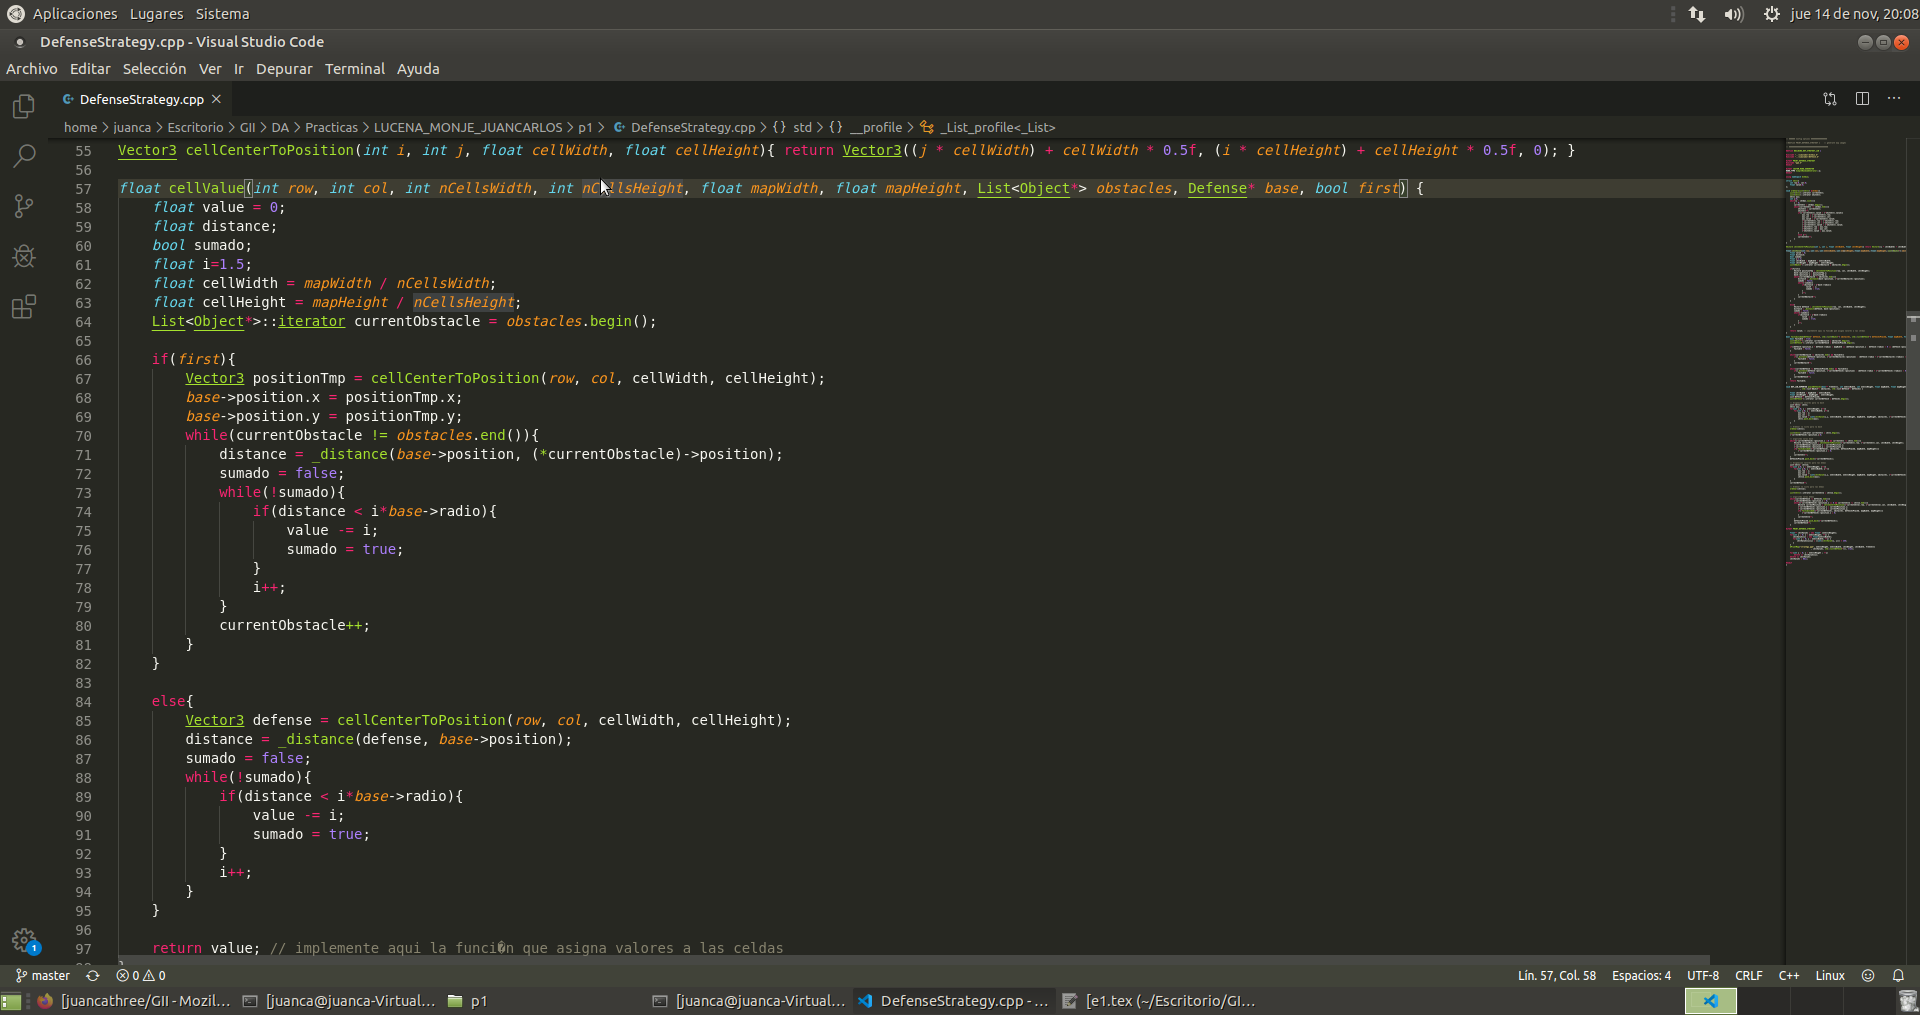
\includegraphics[width=0.7\linewidth]{./defenseValueCellsHead} % no es necesario especificar la extensión del archivo que contiene la imagen
\caption{Estrategia devoradora para la mina}
\label{fig:defenseValueCellsHead}
\end{figure}


\item Implemente su propia versión del algoritmo de ordenación por fusión. Muestre a continuación el código fuente relevante. 

Escriba aquí su respuesta al ejercicio 2.


\item Implemente su propia versión del algoritmo de ordenación rápida. Muestre a continuación el código fuente relevante. 

Escriba aquí su respuesta al ejercicio 3.

\item Realice pruebas de caja negra para asegurar el correcto funcionamiento de los algoritmos de ordenación implementados en los ejercicios anteriores. Detalle a continuación el código relevante.

Una vez haya seleccionado una celda del conjunto si es valida se asigna y ya no puede excluirse y en el caso de que no sea valida no se vuevlve a tener nunca en cuenta.


\item Analice de forma teórica la complejidad de las diferentes versiones del algoritmo de colocación de defensas en función de la estructura de representación del terreno de batalla elegida. Comente a continuación los resultados. Suponga un terreno de batalla cuadrado en todos los casos. 

Escriba aquí su respuesta al ejercicio 5.

\item Incluya a continuación una gráfica con los resultados obtenidos. Utilice un esquema indirecto de medida (considere un error absoluto de valor 0.01 y un error relativo de valor 0.001). Considere en su análisis los planetas con códigos 1500, 2500, 3500,..., 10500. Incluya en el análisis los planetas que considere oportunos para mostrar información relevante.

Escriba aquí su respuesta al ejercicio 6.

\end{enumerate}

Todo el material incluido en esta memoria y en los ficheros asociados es de mi autoría o ha sido facilitado por los profesores de la asignatura. Haciendo entrega de este documento confirmo que he leído la normativa de la asignatura, incluido el punto que respecta al uso de material no original.

\end{document}
